\documentclass[jou]{apa6}

\usepackage[american]{babel}

\usepackage{csquotes}
\usepackage[style=apa,sortcites=true,sorting=nyt,backend=biber]{biblatex}
\DeclareLanguageMapping{american}{american-apa}
\addbibresource{bibliography.bib}


%%%%%%%%%%%%%%%%%%%%%%%%%%%%%%%%%%%%%%%%
%% Discrete Structures
%% The start of RBS stuff
%%%%%%%%%%%%%%%%%%%%%%%%%%%%%%%%%%%%%%%%

% Working internal and external links in PDF
\usepackage{hyperref}
% Extra math symbols in LaTeX
\usepackage{amsmath}
\usepackage{gensymb}
\usepackage{amssymb}
% Enumerations with (a), (b), etc.
\usepackage{enumerate}
\usepackage{xcolor}

\let\OLDitemize\itemize
\renewcommand\itemize{\OLDitemize\addtolength{\itemsep}{-6pt}}

\usepackage{etoolbox}
\makeatletter
\preto{\@verbatim}{\topsep=3pt \partopsep=3pt }
\makeatother

% These sizes redefine APA for A4 paper size
\oddsidemargin 0.0in
\evensidemargin 0.0in
\textwidth 6.27in
\headheight 1.0in
\topmargin -24pt
\headheight 12pt
\headsep 12pt
\textheight 9.19in



\title{Sample Quiz 8}
\author{Discrete Structures, Spring 2020}
\affiliation{RBS}

\leftheader{Discrete Quiz 10}

\abstract{%
}

%\keywords{}

\setlength\parindent{0pt}

\begin{document}

%\thispagestyle{empty}

\twocolumn
\section{Quiz 10: Binary Relations}

\vspace{6pt}
{\bf Question 1}\\
Some people participate in an Einkaufshelden program \textendash{} they 
go to one of the shops $A$, $B$ or $C$ and deliver the products to the endpoints
$X$, $Y$ or $Z$. Each of the $9$ edges is selected by the same probability 
(Figure~\ref{fig:k33-weights})

\begin{figure}[!htb]
\center{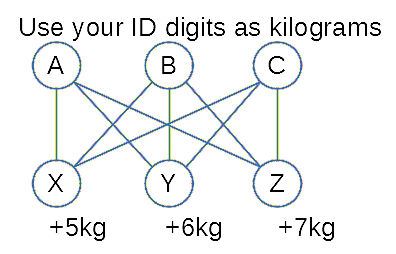
\includegraphics[width=2in]{quiz-10/k33-weights.png}}
\caption{\label{fig:k33-weights} The Paths of a Delivery Service.}
\end{figure}


The sum of the numbers on both ends of an edge shows 
how many kilograms of stuff were delivered. (For example, if your Student ID has 
$A=0$, then on $AZ$ there are $0+7 = 7$ kilograms.
Let $X$ denote the random variable: the kilograms of stuff delivered
on a single edge.

Write the variance $V(X)$ as an irreducible fraction {\tt P/Q}. 


\vspace{6pt}
{\bf Question 2.}\\
Given a set of the first positive integers $S = \{ 1,2,\ldots,A+B+(10-C) \}$
(where {\tt A,B,C} are the digits from your student ID). 
We define a relation on $S$: $aRb$ is true iff $|a - b| \leq 2$.

Let $R^2$ be the second power of that relation $R$ and let $M_{R^2}$
be its matrix. Find the number of 1s in this matrix (In other words: 
how many pairs belong to this relation?)


\vspace{6pt}
{\bf Question 3.}\\
Define a set $S$ of these six positive integers: 
\begin{align}
S = \{ & 1+\mathtt{A},\; 2+\mathtt{A}+\mathtt{B},\; 3+\mathtt{A}+\mathtt{B}+\mathtt{C},\;
4 + 2\mathtt{A}+\mathtt{B}+\mathtt{C},\; \nonumber \\
 & 5 + 2\mathtt{A}+2\mathtt{B}+\mathtt{C},\;
6 + 2\mathtt{A}+2\mathtt{B}+2\mathtt{C}\}. \nonumber
\end{align}

Now compute the remainders of the elements of $S$ when divided by $16$. 
You should get another set $S'$ where each element is between $0$ and $15$. 
($S'$ may contain fewer elements than $S$, if some remainders are identical.)
Let $b_i$ be a sequence of bits ($i = 0,\ldots,15$):
$$b_i = 1\;\text{iff}\;i \in S'.$$

We define a matrix for relation $R$ as follows:
$$M_R = \left( \begin{array}{cccc}
b_{0} & b_1 & b_2 & b_3 \\
b_{4} & b_5 & b_6 & b_7 \\
b_{8} & b_9 & b_{10} & b_{11} \\
b_{12} & b_{13} & b_{14} & b_{15} \\
\end{array} \right)$$
Let $M^{\ast}$ be the matrix of the transitive closure of $R$. 
Find the number of 1s in the matrix $M^{\ast}$.


\vspace{6pt}
{\bf Question 4.}\\
The size of a set $S$ is computed from your ID:
$$|S| = \mathtt{A}+\mathtt{B}+(10 - \mathtt{C}).$$ 
Let $N$ be the number of binary relations on $S$ that are  
reflexive and symmetric at the same time.
Write the last $3$ digits of $N$ in your answer.

{\em Hint} If you need to find the last $3$ digits of some large number, you 
can use periodicity (similar to this: \url{https://bit.ly/33NrJKI}) or Euler's theorem 
(see \url{https://bit.ly/33PyI5Q}) or Chinese Remainder theorem.


\vspace{6pt}
{\bf Question 5.}\\
Find the join of the 3-ary relation:
\begin{verbatim}
{ (Wages,MS410,N507),
  (Rosen,CS540,N525),
  (Michaels,CS518,N504),
  (Michaels,MS410,N510) }
\end{verbatim}
and the 4-ary relation:
\begin{verbatim}
{ (MS410,N507,Monday,6:00), 
  (MS410,N507,Wednesday,6:00), 
  (CS540,N525,Monday,7:30),
  (CS518,N504,Tuesday,6:00), 
  (CS518,N504,Thursday,6:00) }
\end{verbatim}
with respect to the last two fields of the first relation and 
the first two fields of the second relation. 

Write the number records in the join.

\vspace{6pt}
{\bf Question 6.}\\
Let $R$ be a relation on the set $\{x_1,x_2,x_3\}$ that is reflexive and transitive, but not antisymmetric.
Denote its matrix by
$$M_R =  \left( \begin{array}{ccc}
b_{11} & b_{12} & b_{13} \\
b_{21} & b_{22} & b_{23} \\
b_{31} & b_{32} & b_{33} \\
\end{array} \right)$$

If there are multiple answers, write the lexicographically first one.
Write all the 9 bits (as a sequence of 0s and 1s) in your answer: $b_{11}b_{12}b_{13}b_{21}b_{22}b_{23}b_{31}b_{32}b_{33}$.\\
{\footnotesize
\textcolor{red}{The original formulation did not have the lexicographical ordering requirement. Therefore, 
any matrix matching the conditions is fine.}
}




\vspace{6pt}
{\bf Question 7.}\\
Let $R$ be a relation on $\{a, b, c\}$ that is reflexive and transitive, but not symmetric.
Denote its matrix by
$$M_R =  \left( \begin{array}{ccc}
b_{11} & b_{12} & b_{13} \\
b_{21} & b_{22} & b_{23} \\
b_{31} & b_{32} & b_{33} \\
\end{array} \right)$$

If there are multiple answers, write the lexicographically first one. 
Write all the 9 bits (as a sequence of 0s and 1s) in your answer: $b_{11}b_{12}b_{13}b_{21}b_{22}b_{23}b_{31}b_{32}b_{33}$.\\
{\footnotesize
\textcolor{red}{The original formulation did not have the lexicographical ordering requirement. Therefore, 
any matrix matching the conditions is fine.}
}



\newpage

\subsection{Answers}

In solutions we assume that $A = 4$, $B = 5$, $C = 6$. 

\vspace{6pt}
{\bf Question 1.} Answer: {\tt 7} (if $A = 4$, $B = 5$, $C = 6$)\\ 

Figure~\ref{fig:k33-weights-456} shows all the weight combinations in this case. 
The list of total weights on all $9$ edges is the following: 
$$x_1 = 9,\;10,\;11,\;10,\;11,\;12,\;11,\;12,\;x_9 = 13.$$
The mean value is $11$. Variance $V(X)$ is the arithmetic mean of all squared deviations from that mean:
$$V(X) = \frac{\sum_{i=1}^9 (x_i - 11)^2}{9} = \frac{12}{9} = \frac{4}{3}.$$

Therefore $m+n = 4+3 = 7$.

\begin{figure}[!htb]
\center{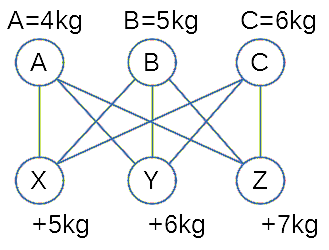
\includegraphics[width=1.6in]{quiz-10/k33-weights-456.png}}
\caption{\label{fig:k33-weights-456} Delivery Service (specific values).}
\end{figure}


\vspace{6pt}
{\bf Question 2.} Answer: {\tt 97} (if $A = 4$, $B = 5$, $C = 6$)\\ 
$S = \{ 1,2,\ldots,A + B + (10-C) \} = \{ 1,2,\ldots,13 \}$,\\
The relation $R^2$ on any two $a,b \in S$ holds, iff 
the distance between $a,b$ is no more than $4$.
This follows from the ``triangle inequality''. 

Namely, $a(R^2)b$ holds, if there exists $c$ that $aRc$ and $cRb$. 
Therefore $|a-c| \leq 2$ and $|c-b| \leq 2$ and we should have 
$|a - b| \leq 4$. The matrix of $R^2$ has $13 \times 13$ entries. 
Out of these entries the main diagonal (where $a=b$) and also 
other diagonal lines that run parallel to that contain $1$s.
The total number of $1$'s is 
$$9 + 10 + 11 + 12 + 13 + 12 + 11 + 10 + 9 = 97.$$







\vspace{6pt}
{\bf Question 3.} Answer: {\tt 16} (if $A = 4$, $B = 5$, $C = 6$)\\ 
Plug in the numbers $A,B,C$: 
$$S = \{ 5, 11, 18, 23, 29, 36 \},$$
$$S' = \{ 5, 11, 2, 7, 13, 4 \},$$
$$M_R = \left( \begin{array}{cccc}
0 & 0 & 1 & 0 \\
1 & 1 & 0 & 1 \\
0 & 0 & 0 & 1 \\
0 & 1 & 0 & 0 \\
\end{array} \right).$$

This matrix only contains $6$ elements equal to $1$, but its transitive
closure is all $16$ elements equal to $1$. Indeed, if we consider the relation $R$ 
on a set of four elements: $A = \{ a_1, a_2, a_3, a_4 \}$, then there is a cyclical path: 
$$a_1Ra_3,\;a_3Ra_4,\;a_4Ra_2,\;a_2Ra_1.$$
Therefore the transitive closure is a relation consisting of all pairs of elements $A \times A$. 



\vspace{6pt}
{\bf Question 4.} Answer: {\tt 544} (if $A = 4$, $B = 5$, $C = 6$)\\ 
We get $|S| =  A + B + (10 - C) = 13$. 
The matrix of any binary relation $R$ defined on $S$ has $13 \times 13 = 169$ elements. 
Since $R$ is reflexive, all the elements on the main diagonal of that matrix are equal to $1$. 
Moreover, any elements above the diagonal are symmetric to some element below the main diagonal. 
Ultimately, we can only choose $(169 - 13)/2 = 78$ elements in the matrix. 
Each element can have two values, therefore $N = 2^{78}$. 

The last three digits in that number are $544$. 
Indeed,
$$\left\{ \begin{array}{l}
2^{78} \equiv 0\; (\text{mod}\; 8), \\
2^{78} \equiv 44\;(\text{mod}\; 125). \\
\end{array} \right.$$

The first congruence is obvious (any large power of $2$ is divisible by $8$). 
The second one follows from 
\begin{align}
2^{78} & = 2^{64} \cdot 2^{8} \cdot 2^{4} \cdot 2^{2} \equiv  \nonumber \\
  & \equiv 116 \cdot 6 \cdot 16 \cdot 4 = \nonumber \\
  & = 44544 \equiv 44 \;(\text{mod}\; 125) \nonumber
\end{align}

\vspace{6pt}
{\bf Question 5.} Answer: {\tt 5}\\ 

{\footnotesize
\begin{tabular}{|l||ll||ll|} \hline
{\bf Table1} & {\bf Joined} &  & {\bf Table2} & \\ \hline
(T1.L1) Wages & MS410 & N507 & (T2.L1) Mon & 6:00 \\ \hline
(T1.L1) Wages & MS410 & N507 & (T2.L2) Wed & 6:00 \\ \hline
(T1.L2) Rosen & CS540 & N525 & (T2.L3) Mon & 7:30 \\ \hline
(T1.L3) Michaels & CS518 & N504 & (T2.L4) Tue & 6:00 \\ \hline
(T1.L3) Michaels & CS518 & N504 & (T2.L5) Thu & 6:00 \\ \hline
\end{tabular}
}

In this table the middle section shows the two joined columns. 
The left section shows the lines from Table 1 (with respective line numbers
in that table). The right section shows the lines from Table 2 (also with line numbers). 


\vspace{6pt}
{\bf Question 6.} Answer: {\tt 100011011}\\ 
We know that the relation is reflexive, so all the elements on its diagonal are $1$
($b_{11} = b_{22} = b_{33} = 1$). 
It must not be antisymmetric, so there must be $x \neq y$ such that $xRy$ and $yRx$. 
Since we want to have the lexicographically first matrix, we set the entries $b_{23}$ and
$b_{32} = 1$. The matrix is now as follows: 

$$M_R =  \left( \begin{array}{ccc}
1 & 0 & 0 \\
0 & 1 & 1 \\
0 & 1 & 1 \\
\end{array} \right)$$

We can easily verify that the relationship $R$ is also transitive (in fact, it is an 
equivalence relationship with two equivalence classes $\{x_1\}$ and
$\{x_2,x_3\}$). 



\vspace{6pt}
{\bf Question 7.} Answer: {\tt 100010011}\\
We know that the relation is reflexive, so all the elements on its diagonal are $1$
($b_{11} = b_{22} = b_{33} = 1$). 
It must not be symmetric, so we can set $b_{23} \neq b_{32}$. (In order to be 
the lexicographically first, we do not want to touch earlier entries in that matrix.)

$$M_R =  \left( \begin{array}{ccc}
1 & 0 & 0 \\
0 & 1 & 0 \\
0 & 1 & 1 \\
\end{array} \right)$$


\end{document}

